\documentclass[a4paper,12pt,french]{article}

\usepackage[cours]{../../Style}

% Début du document
%%%%%%%%%%%%%%%%%%%
\begin{document}

\title{Droites du plan}
\maketitle

\begin{programme}
\item Vecteur directeur d'une droite
\item Equation de droite: Equation cartésienne, \textit{réduite}
\item \textit{Pente (ou coefficient directeur) d'une droite non parallèle à l'axe des ordonnées}
\item Capacités:
\begin{itemize}
\item Déterminer une équation de droite \textit{à partir de deux points}, un point et un vecteur directeur \textit{ou un point et la pente}.
\item Déterminer la pente ou un vecteur directeur d'une droite donnée par une équation ou une représentation graphique
\item Tracer une droite connaissant son équation cartésienne \textit{ou réduite}.
\item \textit{Etablir que trois points sont alignés ou non}
\item Déterminer si deux droites sont parallèles ou sécantes
\item Résoudre un système de deux équations linéaires à deux inconnues, déterminer le point d'intersection de deux droites sécantes
\end{itemize}
\end{programme}

%\begin{FlushLeft}

\section{Equations cartésiennes et réduites}

\section{Vecteur directeur d'une droite}

\section{Intersections et systèmes}



\section{Equation cartésienne de droite et vecteur directeur.}
\begin{defin}
Soit $\mathscr{D}$ une droite, et $A$ et $B$ deux points de $\mathscr{D}$.\\
On appelle \textbf{vecteur directeur} de $\mathscr{D}$ tout vecteurs $\vv{u}$ non nul colinéaire à $\vv{AB}$.\\
\textit{\underline {Autrement dit}: le vecteur $\vv{u}$ donne la direction de la droite $\mathscr{D}$}
\end{defin}

\begin{center}
    
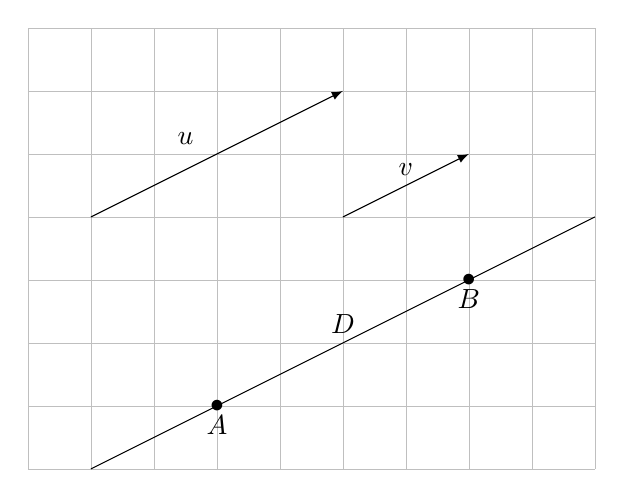
\begin{tikzpicture}[scale=0.8]
    \tkzInit[xmin=-3, xmax=6, ymin=-2,ymax=5]
    \tkzDrawXY
    \draw[lightgray,very thin] (-3,-2) grid (6,5);
    \draw  (-2,-2) -- (6,2);
     \draw [->,>=latex] (-2,2) -- (2,4);
      \draw [->,>=latex] (2,2) -- (4,3);
     \draw (2,0) node [above] {$\mathscr{D}$};
     \draw (0,-1) node {$\bullet$};
     \draw (0,-1) node [below] {$A$};
     \draw (4,1) node {$\bullet$};
     \draw (4,1) node [below]{$B$};
     \draw (-0.5,3) node [above]{$\vv{u}$};
     \draw (3,2.5) node [above]{$\vv{v}$};

\end{tikzpicture}
\end{center}

\begin{rmq}
Un vecteur directeur n'est pas unique: ici les vecteurs $\vv{u}$ et $\vv{v}$ sont des vecteurs directeurs de la droite $(AB)$.
\end{rmq}

\begin{exercice}
Soit \Oij un repère du plan.\\
Donner \textbf{des} vecteurs directeurs des droites $\mathscr{D}{_1}$,$\mathscr{D}{_2}$,$\mathscr{D}{_3}$ et $\mathscr{D}{_4}$.
\end{exercice}


\compo[0.7]{
\begin{center}
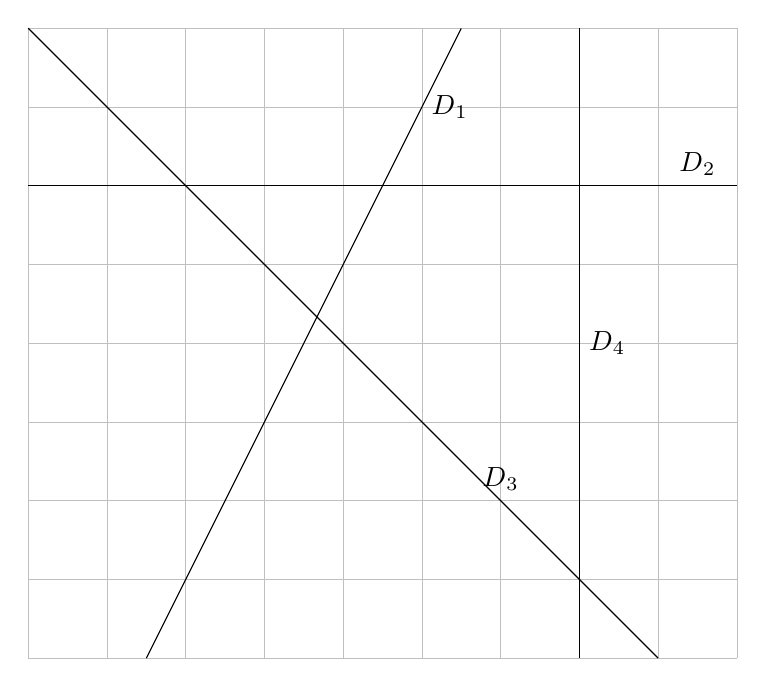
\begin{tikzpicture}[scale=1]
    \tkzInit[xmin=-3, xmax=6, ymin=-2,ymax=6]
    \tkzDrawXY
    \draw[lightgray,very thin] (-3,-2) grid (6,6);
    \draw [domain=-1.5:2.5,samples=100] plot (\x,{2*\x+1});
    \draw [domain=-3:5,samples=100] plot (\x,{-\x+3});
    \draw [-] (-3,4) -- (6,4);
    \draw [-] (4,-2) -- (4,6);
    \draw (2,5) node[right]{$\mathscr{D}{_1}$};
    \draw (3,0) node[above]{$\mathscr{D}{_3}$};
    \draw (5.5,4) node[above]{$\mathscr{D}{_2}$};
    \draw (4,2) node[right]{$\mathscr{D}{_4}$};
\end{tikzpicture}
\end{center}
}{\qrcode[height=2cm]{https://youtu.be/6VdSz-0QT4Y}}


\begin{prop}
Une équation cartésienne de la droite passant par le point $A(x_A;y_A)$ et de vecteur directeur $\vv u \dbinom{-b}{a}$ est de la forme $ax+by+c=0$.
\end{prop}

\begin{fait}
Un point $M(x;y)$ appartient à cette droite ssi $\vv{AM} \dbinom{x-x_A}{y-y_A}$ et $\vv u \dbinom {-b}{a}$ sont colinéaires.\\
Il faut donc que $det(\vv{AM};\vv{u})=0$.\\
Il vient, $$det(\vv{AM};\vv{u})=\begin{vmatrix} x-x_A & -b \\ y-y_A & a \end{vmatrix}=a(x-x_A)-(-b)(y-y_A)=0$$

En développant, l'équation peut s'écrire:

$$ax+by+(-ax_A-by_A)=0$$

On pose $c=-ax_A-by_A$

d'où: $$\boxed{ax+by+c=0}$$

\end{fait}



\begin{cor}
Si les coordonnées $(x;y)$ d'un point $M$ vérifient l'équation $ax+by+c=0$, alors $M$ appartient à la droite dont un vecteur directeur est $\vv u \dbinom {-b}{a}$.
\end{cor}

\begin{exercice}
On considère un repère \Oij du plan.

\begin{enumerate}
    \item Déterminer une équation cartésienne de la droite $\mathscr{D}$ passant par le point $A(3;1)$ et de vecteur directeur $\Coord{u}{-1}{5}$
    \item Déterminer une équation cartésienne de la droite $\mathscr{D'}$ passant par les points $B(5;3)$ et $C(1;-3)$
\end{enumerate}

\end{exercice}

\begin{framed}
\vspace{3cm}
\end{framed}

\section{Systèmes de deux équations à deux inconnus}

Résoudre un système à deux inconnues , c'est trouver le ou les couples $(x;y)$ qui vérifie(nt) à la fois les deux équations.

\begin{exercice}
Montrer que le couple $(2;3)$ vérifie le système d'équations:

\[
\left \{
\begin{array}{c c}
    5x-2y=4 \\
    -x+y=1
\end{array}
\right.
\]

\end{exercice}

\begin{framed}
\vspace{3cm}
\end{framed}

\subsection{Résolution graphique}

On se ramène à deux équations de droites que l'on trace.\\
L'unique solution du système est alors les coordonnées du point d'intersection des deux droites.

\begin{exercice}
Tracer les droites du système puis trouver les coordonnées du point d'intersection.
\[
\left \{
\begin{array}{c c}
    5x-2y=4 \\
    -x+y=1
\end{array}
\right.
\]


\begin{center}
    

 
\begin{tikzpicture}[scale=0.8]
    \tkzInit[xmin=-4, xmax=6, ymin=-2,ymax=6]
    \tkzDrawXY
    \draw[lightgray,very thin] (-4,-2) grid (6,6);
    
\end{tikzpicture}
\end{center}



\end{exercice}


\subsection{Résolution algébrique}




\subsubsection{Méthode par combinaison linéaire}

\begin{exercice}

Résoudre dans $\R$ le système suivant:


\[
\left \{
\begin{array}{c c}
    2x-3y=9 \\
    2x+y=-1
\end{array}
\right.
\]


\end{exercice}

\begin{framed}
\vspace{7cm}
\end{framed}


\subsubsection{Méthode par substitution}

\begin{exercice}

Résoudre dans $\R$ le système suivant:


\[
\left \{
\begin{array}{c c}
    6x-7y=1 \\
    x-3y=-2
\end{array}
\right.
\]



\end{exercice}

\begin{framed}
\vspace{7cm}
\end{framed}

\end{document}
